\chapter{Introduction}
\label{chapter:introduccion}

\textit{Not Final Note: \TBD{This color ('TBD' tag in latex) are going to be used in non-final versions of the memory to highlight the non-final sentences or things to be changed in the final version}}.

In this chapter we will introduce the main background, and aims of the project, basing it on its non-solved tasks and relevance.

%%% SECTION
\section{Problem overview and relevance}

\subsection{MRI general problems}

Neuroimaging in medicine allows studying the morphological features of the human brain. With the objective of improving the detection systems, diagnostic and treatment, correlations between the morphological features and the neurological disorders can be addressed in order to achieve that \cite{abou2006neuroimaging}. If we improve brain magnetic resonance image analysis \ref{fig:figs/MRI_image.jpg}, we will improve the detection systems and treatments for neurological diseases, so the social relevance of the field is very important.

\imagen{figs/MRI_image.jpg}{Brain MRI examples \cite{fotomri}}

The relevance of the project is also shown that there are a lot of branches in which neuroimaging analysis can improve. Machine learning, and more recently Deep Learning and Computer Vision, has irrupted in this field for helping in some tasks: 

\begin{itemize}
    \item \textbf{Disease detection: segmentation and classification}. There are still several problems to solve in classification and segmentation problems. Brain MRIs are high dimensional, so we have to recruit big amount of images to properly develop a Machine Learning model that be able to achieve high accuracy. It is very difficult to recruit a large number of images, especially disease images. Even if it performs well, machine learning algorithms have been criticized due to the difficult of extract a clear knowledge of them (black-boxes).  \cite{myronenko20183d}. So a experimental approach is disease detection based on outliers from a normative model. Patients with pathologies will be outliers in the distribution build by the normative model (they will be out of normal range defined by the normative model) \cite{marquand2016normative} \cite{mourao2011outlier}. It could be seen as an unsupervised anomaly detection technique, in which we don't need labeled data.
    \item \textbf{Data Augmentation}. Lack of data problem can be addressed by Data Augmentation techniques, which look for improve our Machine Learning models \cite{GanDataAugment2018} and robustness of pipelines \cite{2020inpainting}.
    \item \textbf{Improvement of data acquisition}. Recently high-impact \myurl{https://fastmri.org/}{FastMRI} release from Facebook for improving the speed in MRI scans \cite{fastmri}.
    \item \underline{\textbf{Image enhancement}}. Clinical evaluation is critical for good disease treatment. Experts and algorithms need good quality images to carry out their tasks. This is a problem we want to address, so we will explain it deeper in the document \cite{tamada2020review} \cite{myronenko20183d}. 
\end{itemize}

However, some of these problems overlap. The advance in some of them leads to the advance in another. \textbf{Image reconstruction}, which is a mainly sub-problem of image enhancement, could help to achieve better results in data acquisition (i.e. reconstruct the image from less data collected), unsupervised anomaly detection (i.e. reconstruction of the disease image differs more than the pathology-free one), data augmentation (i.e. reconstruction from patholohy-free to abnormal and viceversa) and, obviusly, image enhancement (i.e. reconstruction of cropped parts or reconstruction without noise and artifacts). \textbf{Thus, the main purpose for this project is to apply this reconstruction techniques for noise reduction (image enhancement) and data augmentation (lesion inpainting),} being another applications discussed for future work.

\subsection{MRI Image enhancement}

\textbf{We are going to focus on the problem of image enhancement, specifically the problem of image reconstruction}. With this reconstruction technique, the noise and artifacts will be reduced, see \ref{fig:figs/Denoised_MRI.jpeg}, and the image quality will be improved. If we achieved good performance in this task, we would research about how to apply this solution to unsupervised disease detection or data augmentation.

\imagen{figs/Denoised_MRI.jpeg}{Noised and Denoised MRI \cite{fotoDenoisedMri}}

Magnetic resonance images are collected with MR scans and the scan process, even though it is improved continually, adds some failures to the MR image. MR images have some random \textbf{noise} and \textbf{artifacts} due to this fact \cite{artifacts86}. This noise and artifacts are present in the image due to different reasons: hardware-reasons (magnetic fields, etc.), body motion during scanning, thermal noise, weak signal intensity (which causes low signal-to-noise ratio), etc. The difference between noise and artifact is that noise can hide the characteristics of an image, whereas artifacts appear to be characteristic but are not. If the 'problem' is structured, it is probably an artifact, while if it is random, it is probably noise.

\subsection{Noise and artifact reduction with Deep Learning}

Noise and artifact reduction is one of the main principal problems which are classically solved with \underline{reconstruction} techniques. To address this problem many approaches have been done, all of them with some disadvantages. Advanced filtering methods \cite{filtermeth12} or retrospective correction approaches have been proposed, but, with the rise of \textbf{Deep Learning}, other methods have been proposed that take advantage of this approach. Deep Learning is very powerful in high-dimensional spaces and non-linear problems, so it can make a better job in feature extraction or information compression. Therefore, it will have good performance with images, where the \textbf{underlying structure of the images will be captured and foreign elements such as noise or artifacts can be eliminated through a noise-free reconstruction}. 

There are some approaches to reduce the noise and artifacts in MRI images. An recent and outstanding review is made by D.Tamada \cite{tamada2020review}. In this paper D.Tamada summarize Deep Learning Architectures and applications to MRI. We notice the big relevance of denoiser MRI Deep Learning methods in this review. Although there are many methods, we will focus in brain MRI denoisers. A compilation of articles related with noise reduction is made in table \ref{table:paper_overview}.

There are some Deep Learning Architectures to address in the problem of denoise an brain MRI: Single-scale CNN, Denoising CNN, Autoencoders, and GAN-based architectures. \textbf{We will choose the Autoencoder Architecture for this project}.

\textbf{Autoencoders} \cite{autoencoder} encode the input into a lower-dimensional space. It extracts important information from the higher-dimensional space, encodes it, and then decodes it to reconstruct the higher-dimensional spacer from the lower one. \TBD{This architecture will be deeply explained in \ref{chapter:theory} in further stages of the project.}



\subsection{Our approach}

\begin{tcolorbox}
In this project, we will design a \textbf{Deep Learning autoencoder for reconstructing brain magnetic resonance images reducing noise/artifacts and inpainting lessons, and study its further implications and applications like  data augmentation, disease detection or data acquisition improvement. In other words, we will train a autoencoder with disease-free neuroimaging data and, with this trained autoencoder, we could define a distribution (or normal range) for the neuroanatomical variability for the illness absence with the potential purpose of removing noise or look for diseases. Once trained, the autoencoder should be able to encode a input image and reconstruct it without the noise or lesson.}
\end{tcolorbox}

We want to highlight one main fact: the autoencoder do not remove noise or inpaint a lessons because it is trained like a denoiser or a image-filler. It do reconstruct MRI without noise or lessons because it is trained only with 'clean' and control MRI like target images, so it does not know how to reconstruct noise or lessons. Therefore, once the MRI is encoded in the latent space, the decoder will reconstruct a control clean MRI from this latent space.

\textbf{If the main objective of the project is completed, we could research the application of this model in data augmentation and disease detection fields}. In the case of \textbf{data augmentation}, we will then attempt to reconstruct magnetic resonance images from patients with brain pathologies, with a further view to using the autoencoder to generate 'pathology-free' versions of the said images. In the case of \textbf{disease detection}, we could take an approach like the one in \cite{pinaya2019} (creating a measure for the difference between input and output image and classify it as healthy or non-healthy based on this measure). Patients with pathologies will be outliers in the distribution build by the autoencoder (they will be out of normal range defined by the autoencoder) \cite{marquand2016normative} \cite{mourao2011outlier}. This assumption of patients as outliers (based in \cite{mourao2011outlier}) is used in \cite{pinaya2019} for abnormal brain structure detection.

Of course, we will need \textbf{data}. For this project, we will use \textbf{T1-weighted MRI images of control subjects} (no disease). As the project is of fairly limited length, we won't need to detect disease as a principal objective, but only learn to reconstruct normal MRI images, so we won't need pathology images for this project. In addition, we will investigate whether our method of reconstruction can filter out noise and/or artefacts. So, in essence, we will have $n$ 3D MRI volumes ($n$ can be any number greater than 100) from healthy subjects, we will preprocess it (data augmentation based on adding noise, remove parts...), and train our model to reconstruct the source MRI volumes. We will have access magnetic brain resonance images from control subjects for training the autoencoder. This data is arranged from different sources. We will use a set of T1 weighted control brain MR images for training the autoencoder. Then, we will consider to use another datasets in the experimentation stage:

\begin{itemize}
    \item The \myurl{https://brain-development.org/ixi-dataset/}{IXI dataset} for training.
    \item Other data sources such as \myurl{https://openneuro.org}{Open Neuro} for experiment with autoencoder applications (reconstruction from disease image, etc).
\end{itemize}



\section{Personal motivation}

My personal motivation to carry out the project arises from several factors. My first steps in the world of Machine Learning were in the last year of my career at the University of Burgos. I was lucky enough to collaborate last year with the \myurl{http://admirable-ubu.es/}{ADMIRABLE} research department. The project that I did (in which we continue working) was on the \myurl{https://adrianarnaiz.github.io/TFG-Neurodegenerative-Disease-Detection/}{use of biomarkers extracted from the voice for the construction of classifiers that detect Parkinson's disease}. The project include topics like \textbf{signal processing}, \textbf{supervised learning}, \textbf{unsupervised learning} and \textbf{transfer learning}. The project was very successful and we had a lot of impact at that time. We are currently in the process of meeting with the Burgos hospital to continue developing the model and the application (project and impact recompilation in \myurl{https://github.com/AdrianArnaiz/TFG-Neurodegenerative-Disease-Detection}{Github}).

This project has fully opened me the doors the world of artificial intelligence and machine learning, which is a field of knowledge that I love. I have always liked math, problem-solving and since I started my career I love programming. Therefore, I find this field the ideal that aligns with my tastes and interests. As I said before, I have done lot of jobs with supervised learning or data analysis, but only with tabular data sets or text-datasets, so I wanted to break in the world of image processing and Deep Learning.

Then I worked half year in Ernst and Young, developing Machine Learning systems for RPA tasks (classify emails at Telefónica, Chatbot for Maxium or Fuzzy Name Matching for Xunta de Galicia).

In addition, I believe that the application of AI to medicine is one of the fields that may be of greater general interest to society. By advancing in the speed and quality of medical diagnoses and treatments, it will be possible to achieve health of higher quality, speed and accessibility for all. Also, computer vision and deep learning have helped to achieve big advances in this field nowadays. 


\iffalse
\section{Latex Examples}

\begin{figure}
	\centering
	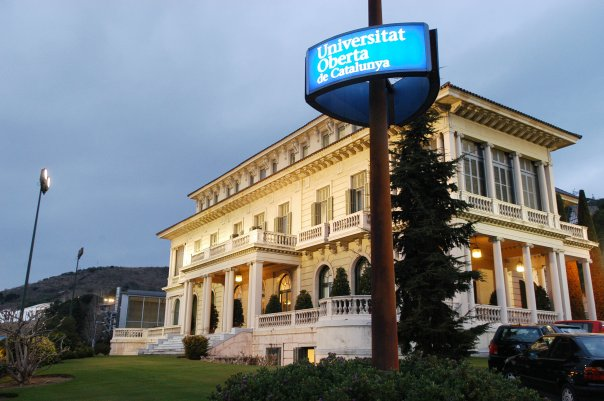
\includegraphics[width=0.6\textwidth]{figs/image1.png}
	\caption{Pie de la imagen.}
	\label{fig:context-anoni1}
\end{figure}


\imagen{figs/image1.png}{asdasd}

Un ejemplo de pseudo-código se puede encontrar en el Código \ref{code:RandomSwitch-1}

\begin{algorithm}
	\caption{Pseudocódigo del algoritmo \textit{Random Switch}}
	\label{code:RandomSwitch-1}
	\begin{algorithmic}
		\REQUIRE{El grafo original $G$ y el porcentaje de anonimización $p$ que se desea aplicar.}
		\ENSURE{El grafo $G$ anonimizado.}
		\STATE $num = round(G.num\_edges() * p)$
		\STATE $i = 0$
		\WHILE {$i < num$}
		\STATE {$e_{1} = G.random\_edge()$}
		\STATE $e_{2} = G.random\_edge()$
		\STATE $new\_e_{1} = (e_{1}.origen, e_{2}.origen)$
		\STATE $new\_e_{2} = (e_{1}.destino, e_{2}.destino)$
		\IF {$!G.exist(new\_e_{1})$ \AND $!G.exist(new\_e_{2})$}
		\STATE $G.add\_edge(new\_e_{1})$
		\STATE $G.add\_edge(new\_e_{2})$
		\STATE $G.delete\_edge(e_{1})$
		\STATE $G.delete\_edge(e_{2})$
		\STATE $i=i+1$
		\ENDIF
		\ENDWHILE
		\RETURN $G$
	\end{algorithmic}
\end{algorithm}

Un ejemplo de tabla se puede ver en la Tabla \ref{table:ejemplo_vertex_refi_query}

\begin{table}
	\centering{}
	\begin{tabular}{ l || c | c | l }
		\hline
		Node ID & $\mathcal{H}_{0}$ & $\mathcal{H}_{1}$ & $\mathcal{H}_{2}$ \\
		\hline
		\hline
		Alice & $\epsilon$ & 1 & \{4\}  \\
		\hline
		Bob & $\epsilon$ & 4 & \{1, 1, 4, 4\}  \\
		\hline
		Carol & $\epsilon$ & 1 & \{4\}  \\
		\hline
		Dave & $\epsilon$ & 4 & \{2, 4, 4, 4\}  \\
		\hline
		Ed & $\epsilon$ & 4 & \{2, 4, 4, 4\}  \\
		\hline
		Fred & $\epsilon$ & 2 & \{4, 4\}  \\
		\hline
		Greg & $\epsilon$ & 4 & \{2, 2, 4, 4\}  \\
		\hline
		Harry & $\epsilon$ & 2 & \{4, 4\}  \\
		\hline
	\end{tabular}
	\caption{\textit{Vertex refinement queries}.}
	\label{table:ejemplo_vertex_refi_query}
\end{table}
\fi